\definecolor{exxetagray}{gray}{0.75}
\definecolor{itemcolor}{RGB}{179,217,255}
\definecolor{usercolor}{RGB}{255,204,179}

\shorthandoff{"}
\chapter{Verwandte Arbeiten}
\label{ch:verwandte_arbeiten}
In der Literatur existieren bereits einige Arbeiten, die sich mit der Berücksichtigung wechselseitiger Präferenzen in der Empfehlungserstellung beschäftigen.
Auch der Bereich der multi-kriteriellen Empfehlungssysteme wurde in der Literatur in diversen Veröffentlichungen behandelt.
Nachfolgend werden verwandte Arbeiten zu reziproken Empfehlungssystemen sowie zu multi-kriteriellen Empfehlungssystemen mit Bezug auf die vorliegende Domäne angeführt.

GLIEDERUNG DIESES KAPITELS ANPASSEN -> Zusammenspiel aus multi-criteria und reciprocal recommender

\section{Reziproke Systeme}
Gemäß \textcite[S. 1467]{yildirim:article} hat die wechselseitige Empfehlung in der Literatur bis heute aufgrund fehlender öffentlicher Datensätze mit Angaben zu Präferenzen der Nutzer eines Netzwerks wenig Aufmerksamkeit erhalten. 

Die erste Veröffentlichung in der Literatur zu wechselseitigen Empfehlungssystemen stammt von \textcite[S. 1ff.]{pizzato:inproceedings}, welche ein wechselseitiges Empfehlungssystem für Online-Dating-Plattformen vorstellen \cite[S. 1469]{yildirim:article}.
Die Autoren beschreiben eine reziproke Empfehlung als eine Linearkombination aus dem Wert der Präferenz eines Nutzers für ein Element ($P1$) und dem Wert der Präferenz eines Elements für einen Nutzer ($P2$):
\begin{equation}\label{eq32}
    PRR(c,s) = w_{1}P1(c,s) + w_{2}P2(c,s)
\end{equation}
Über die Gewichte $w_{1}$ und $w_{2}$ können den Präferenzen von Nutzern bzw. Elementen unterschiedliche Wichtigkeit zugeteilt werden.
% erste referenz zu reciprocal recommendation by pizzato kurz anfüren (siehe S. 1469, file:///C:/Users/masc6/Downloads/1-s2.0-S2215098621000744-main.pdf)
% Darstellung der gewichtung der Präferenzen als linearkombination
% d.h. wie sehr zwei personen übereinstimmen, beides gleich gewichtet
% Dual perspektive graph representation hier: S. 104, file://wsl%24/Ubuntu/home/masc6/Projects/masterarbeit/literatur/recsys%202022%20modeling%20two%20way%20selection%20preference%20for%20person%20job%20fit.pdf

% präferenz eines nutzers höher gewichtet als präferenz der empfohlenen Elemente
% feature optionen können 3 unterschiedliche stadi annehmen. -> classification (label mit match und kein match) S. 68, file://wsl%24/Ubuntu/home/masc6/Projects/masterarbeit/literatur/DiazMetzlerAmer-Yahia%20-%20Relevance%20and%20Ranking%20in%20Online%20Dating%20Systems%20(2010)%20-%200.pdf
% Johannes Thesis

\section{Multi-kriterielle Systeme}
hier bsp anführen für arbeiten die sich mit mk systemen beschäftigen in den 3 bereichen
% Hier erwähnen, dass nicht alle systeme auch als mk-systeme bezeichnet sind, die solche Ansätze anwenden (bspw. hybride systeme)
% Hier erwähnen, dass Fokus auf aggregation mehrerer Kriterien und deren gewichtung liegt -> hiernach suchen

% Verwendung von MAUT (siehe S. 432, file://wsl%24/Ubuntu/home/masc6/Projects/masterarbeit/literatur/Analysis%20and%20Classification%20of%20Multi-Criteria.pdf)
% MAUT in utility based recommenders: file://wsl%24/Ubuntu/home/masc6/Projects/masterarbeit/literatur/Designing%20utility-based%20recommender%20systems%20for%20e-commerce.pdf

\subsection{Multi-attribut basierte Systeme}
% hybrid recommender: weighted -> S. 339, https://link.springer.com/content/pdf/10.1023/A:1021240730564.pdf?pdf=button

\subsection{Multi-objektive Systeme}
% multi-objective example: S. 237, file://wsl%24/Ubuntu/home/masc6/Projects/masterarbeit/literatur/Adaptive%20multi%20attribute%20diversity%20for%20recommender%20systems.pdf

% Bsp im Bereich Reciprocal recommendation: file:///C:/Users/masc6/Downloads/1-s2.0-S2215098621000744-main.pdf
% HIER WEITERMACHEN

Als multi-objektiv bezeichnen \textcite[S. 12]{rodriguez:inproceedings} ihren Ansatz zur Integration "äußerer Merkmale"\footnote{"extraneous features" - \textcite[S. 12]{rodriguez:inproceedings}} in ein semantisches Modell im Bereich des Online-Recruitments. 
Dieser ist in Abbildung \ref{fig:relatedwork:abb1} dargestellt.

\begin{figure}[H]
    \centering
	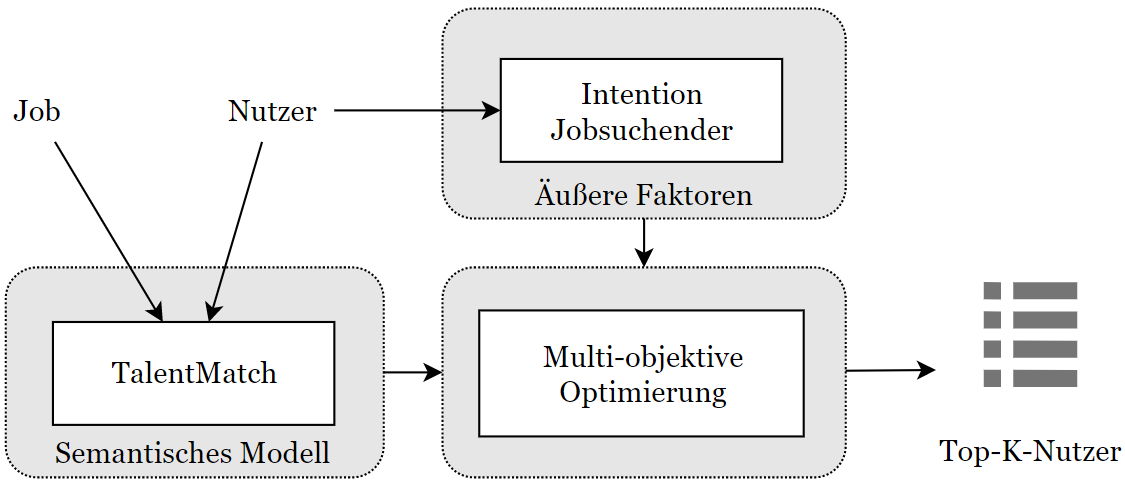
\includegraphics[width=0.9\textwidth]{gfx/talentMatch.png}
	\caption[Ansatz für die Integration äußerer Merkmale in semantische Modelle]{Ansatz für die Integration äußerer Merkmale in semantische Modelle\\
    (Eigene Darstellung in Anlehnung an \cite[S. 12]{rodriguez:inproceedings})}
	\label{fig:relatedwork:abb1}
\end{figure}

Im Detail stellen die Autoren eine Erweiterung des bestehenden \textit{TalentMatch}-Systems des sozialen Netzwerks LinkedIn vor, welche neben des semantischen Matches \cite[S. 2]{jannach:2:inproceedings} zwischen einer Person und einem Job (Objective 1) zusätzlich die Offenheit einer Person für einen Jobwechsel (Objective 2) in die Empfehlungserstellung (Ranking) miteinbezieht.
Dabei gehen die Autoren davon aus, dass die beiden Ziele möglicherweise miteinander konkurrieren, d.h. dass eine Person, die am besten auf eine Jobbeschreibung zutrifft, möglicherweise nicht offen für eine neue Stelle ist.
\textcite[S. 12]{rodriguez:inproceedings} untersuchen in ihrer Arbeit, ob die Berücksichtigung der Neigung von Personen für offene Jobpositionen den Nutzen der Nutzer des Systems dennoch positiv beeinflusst.
Den Nutzen operationalisieren die Autoren als das Engagement zwischen Jobsuchenden und Anbietern von Jobpositionen \cite[S. 14]{rodriguez:inproceedings}, welche diese über Menge aktiver, passiver und inaktiver Nutzer in dem System messen.
Die Integration der Berücksichtigung in das semantische Modell führen \textcite[S. 15]{rodriguez:inproceedings} systematisch über ein Re-Ranking durch.
Dies realisieren die Autoren über folgende Verlust-Funktion $L$ \cite[S. 13]{rodriguez:inproceedings}:
\begin{equation}\label{eq30}
    L(\alpha ,\beta) = -g(f(Y, X, [\alpha , \beta])) + \lambda \Delta (\pi (Y), \pi (f(Y,X,[\alpha ,\beta])))
\end{equation}
Nach \textcite[S. 15]{rodriguez:inproceedings} gibt Funktion $g$ die durchschnittliche Anzahl aktiver und passiver Nutzer in dem erweiterten System $f(Y, X, [\alpha , \beta])$ aus und $\Delta$ die Abweichung des Rankings $\pi (f(Y,X,[\alpha ,\beta]))$ des erweiterten Systems von dem Ranking $\pi (Y)$ des ursprünglichen semantischen Modells.
$\lambda$ stellt einen positiven Trade-Off-Parameter dar \cite[S. 13]{rodriguez:inproceedings}.
% \textcite[S. 13]{rodriguez:inproceedings} merken an, dass die Verlust-Funktion auch als Maximierungsproblem der Funktion $g$ dargestellt werden kann, welches $\Delta$ durch das Aufstellen einer Bedingung $c$ (d.h. $\Delta (\pi (Y), \pi (f(Y,X,[\alpha ,\beta]))) \leq c$) begrenzen kann.
Die Anpassung eines semantischen Matches $y$ realisieren \textcite[S. 15]{rodriguez:inproceedings} durch einen sogenannten "Boost", wobei zwischen einem Boost für aktive ($\alpha$) und passive ($\beta$) Nutzer unterschieden wird:
\begin{equation}\label{eq31}
    f(y,x,[\alpha ,\beta]) = y \times (\alpha^{1\{{x == \textnormal{active}\}}}) \times (\beta^{1\{{x == \textnormal{active}\}}})
\end{equation}
Hierbei ist $1\{x == \textnormal{active}\}$ gleich $1$, wenn die Bedingung innerhalb der geschweiften Klammer wahr ist und $0$ andernfalls.
Das Optimieren der Parameter $\alpha$ und $\beta$ führen \textcite[S. 15]{rodriguez:inproceedings} über eine Rastersuche durch.

\textcite[S. 15f.]{rodriguez:inproceedings} prüften ihren Ansatz anhand von 760 offenen Jobangeboten, von denen jedes zwischen 6 und 9000 mal in Empfehlungen auftauchte.
Dabei stellten die Autoren fest, dass eine signifikante Verbesserung des Nutzens mit einer akzeptablen und vorhersebaren Verschlechterung der semantischen Matches erreicht werden konnte \cite[S. 11]{rodriguez:inproceedings}.
% Dabei stellten die Autoren fest, dass bis zu einem gewissen Wert für Delta ein linearer Zusammenhang zwischen dem Zugewinn an durchschnittlich aktiven und passiven Nutzern und der Aufgabe von Übereinstimmung der Rankings besteht \cite[S. 16]{rodriguez:inproceedings}.
% Für bestimmte Kombinationen von $\alpha$ und $\beta$ konnte die Anzahl aktiver und passiver Nutzer in dem Top-K-Ranking durch Anwendung des erweiterten Modells verdoppelt werden, ohne massive Einbußen in den semantischen Matches einzufahren.
Kritisch betrachten \textcite[S. 16]{rodriguez:inproceedings} an ihrem Ansatz, dass für die Wirksamkeit eines Modells im praktischen Einsatz überprüft werden muss, ob die durchschnittliche Anzahl aktiver und passiver Nutzer tatsächlich repräsentativ für das Engagement von Nutzern in einem System ist.

\subsection{Multi-kriterielle Bewertungen in Empfehlungssystemen}
% Erfinder des aggregation Funktion approaches: file://wsl%24/Ubuntu/home/masc6/Projects/masterarbeit/literatur/New_Recommendation_Techniques_for_Multicriteria_Rating_Systems.pdf
% Arbeit von Jannach wie hier beschrieben mit SVM: S. 102, file://wsl%24/Ubuntu/home/masc6/Projects/masterarbeit/literatur/E-Commerce.pdf
% multi-kriteria: Aggregation function approach: file://wsl%24/Ubuntu/home/masc6/Projects/masterarbeit/literatur/Recommending%20Hotels%20based%20on%20Multidimesional%20Customer%20Ratings.pdf
% ansatz von Tang: zusammenfügen mehrere feature bewertungen, sowie durchschnittsbewertung und kommentare, file:///C:/Users/masc6/Downloads/tdladmin,+TangandMcCalla_JoDI_final.pdf
% Slope one algorithmus und adaptive genetic algorithm von Hassan, S. 327, file://wsl%24/Ubuntu/home/masc6/Projects/masterarbeit/literatur/Imrpoving%20Prediction%20accuracy%20of%20multi-criteria%20recommender.pdf
% Liu et al.: Cluster von Nutzern, welche wichtigkeit einzelner Attribute angeben, zusammenfassung siehe hier S. 4, file:///C:/Users/masc6/Downloads/79_HDIOUD.pdf
% CCSD method, siehe: file:///C:/Users/masc6/Downloads/79_HDIOUD.pdf
% Wenn viele features: liwei et al (zsfsg. siehe hier: file://wsl%24/Ubuntu/home/masc6/Projects/masterarbeit/literatur/A%20Multi-criteria%20Recommender%20System%20Incorporating%20Intensity%20of%20Preferences.pdf )

% was gibt es also nicht? -> Reziprozität als gewichtetes Kriterium (Präferenz der empfohlenen Person zählt nicht genauso viel wie Präferenz des Nutzers, kann daher als gewichtetes Kriterium einer Aggregation Function betrachtet werden, welche über historische daten erlernt werden kann)
% Neue anwendungsbereiche von multi-kriteriellen EMpfehlungen in domänen wie online dating: zitat von S. 553, file://wsl%24/Ubuntu/home/masc6/Projects/masterarbeit/literatur/Towards%20the%20Next%20Generation%20of%20Multi-Criteria%20Recommender.pdf

 \shorthandon{"}